\vspace{-2mm}
\section{实验}
\label{sec:experiments}

\begin{figure*}[!t]
    \centering
    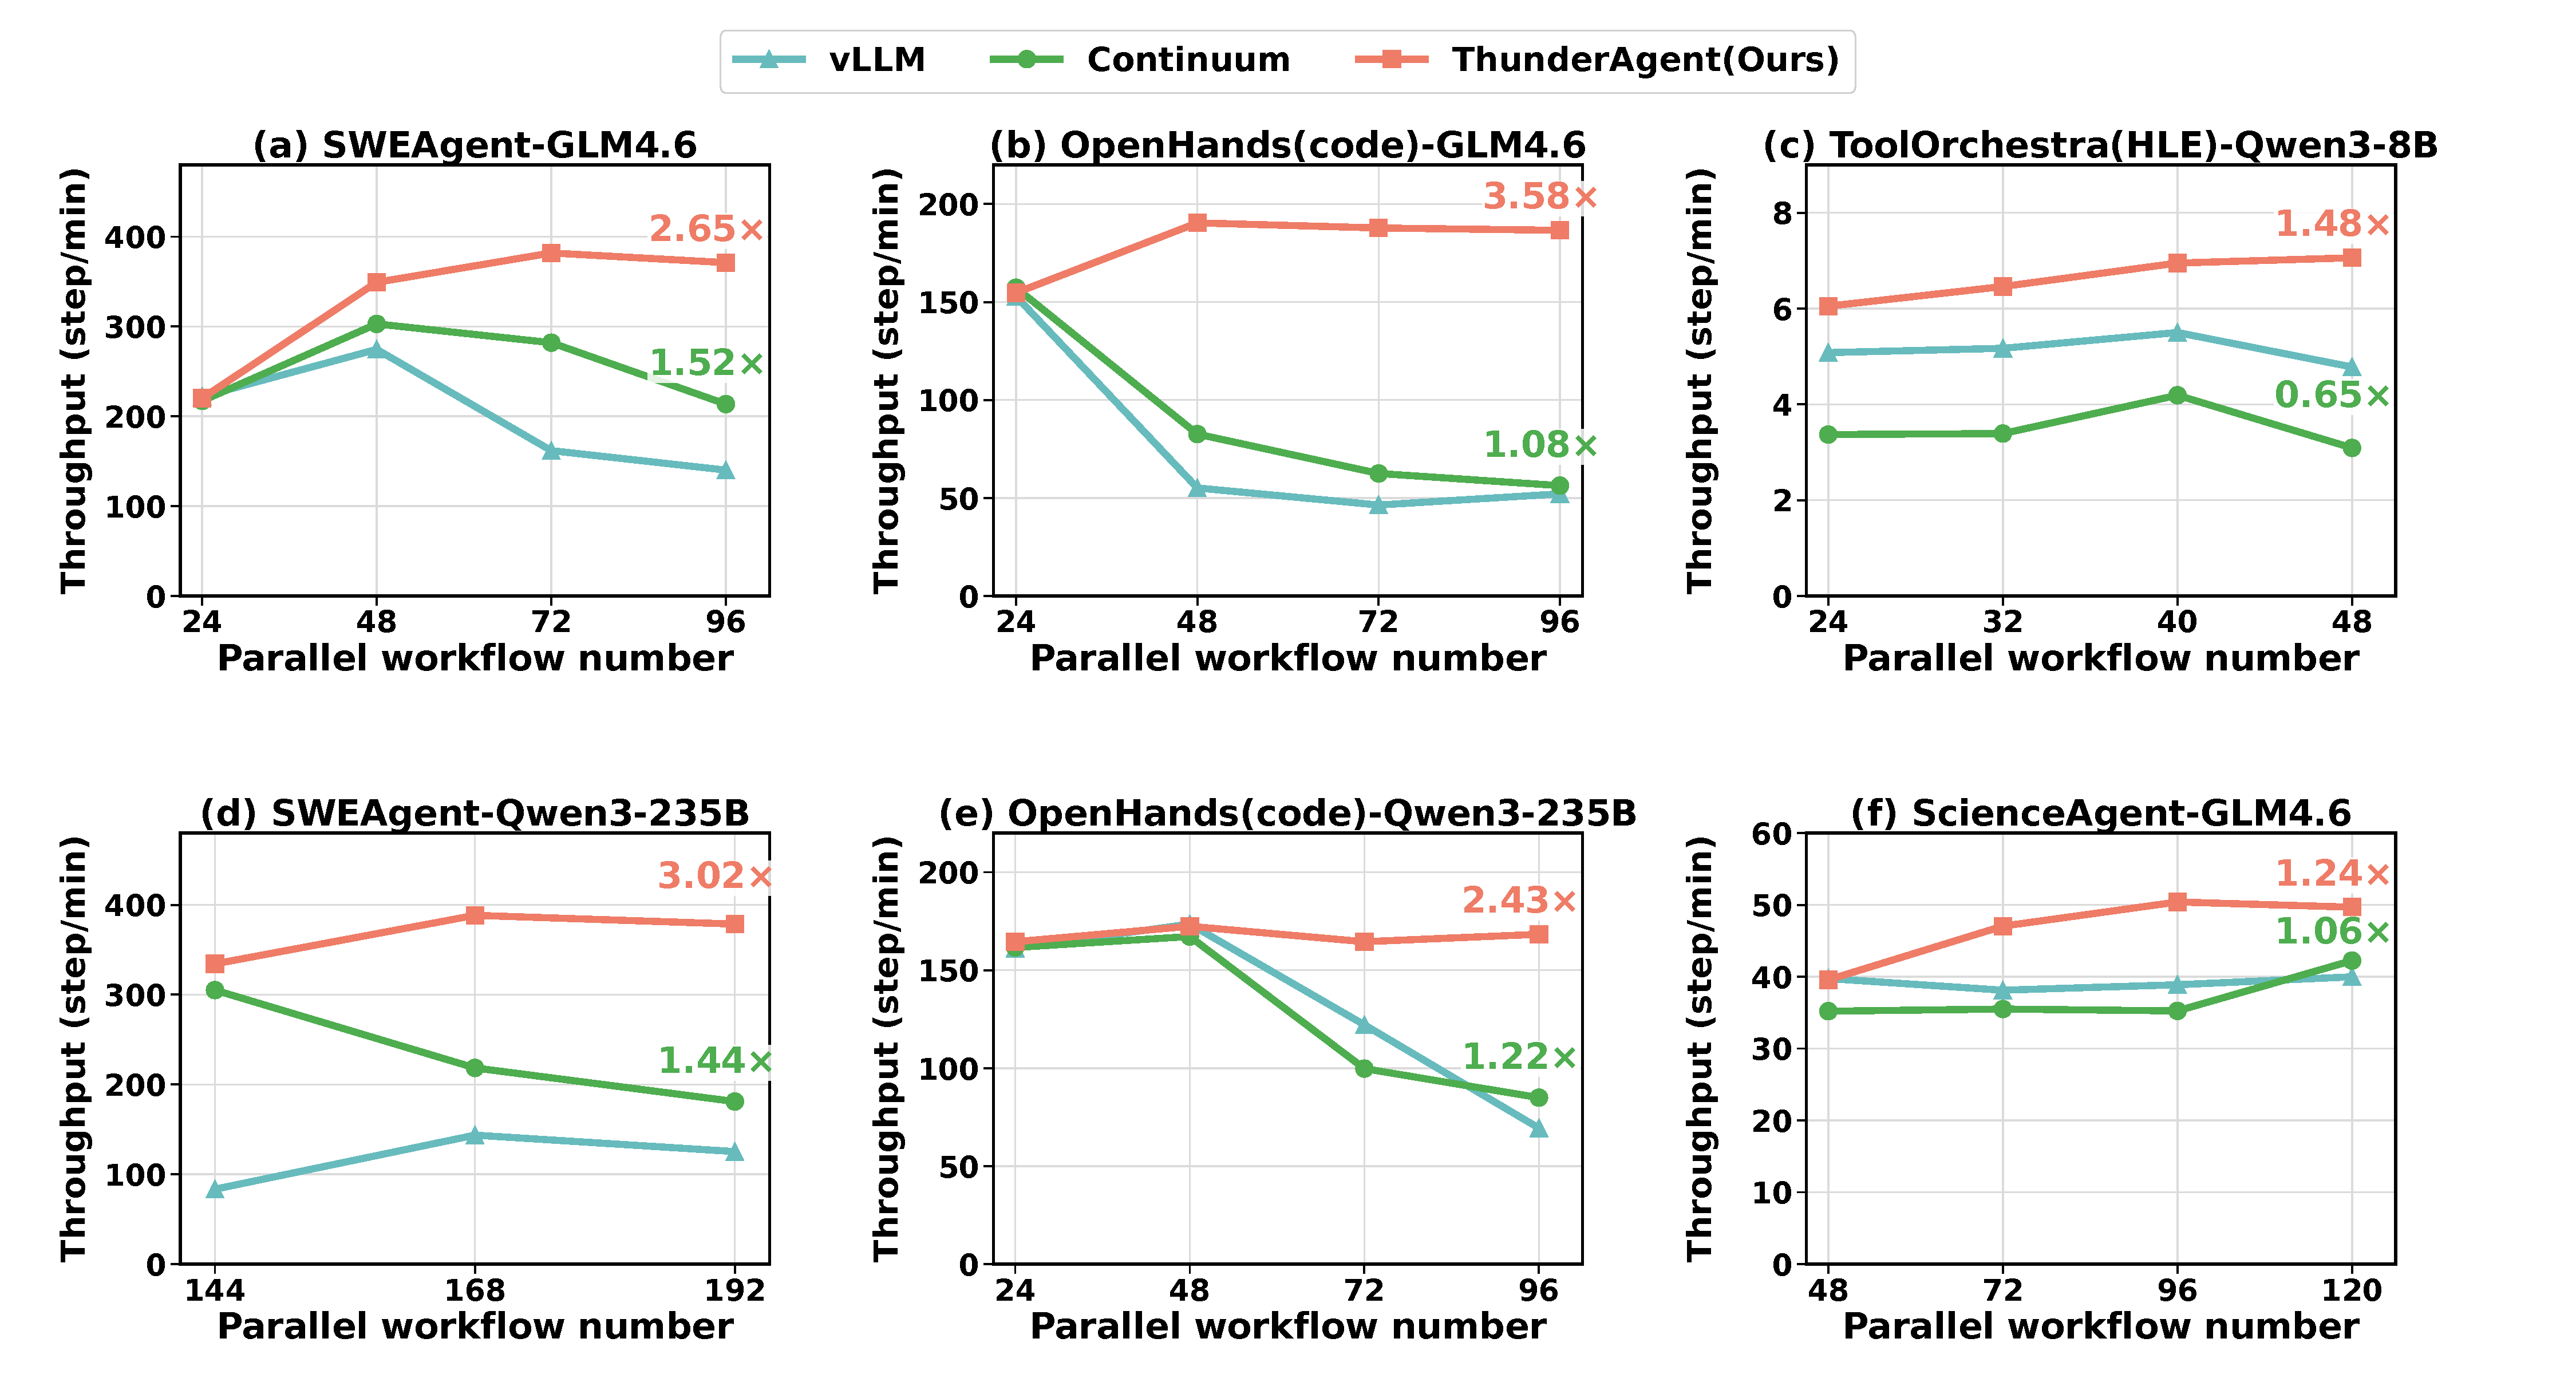
\includegraphics[width=1.0\columnwidth]{Figures/infer_eval.pdf}
    \caption{\textbf{服务评估结果。} \ouralg 在三个模型、四个智能体工作流和三个数据集上，其性能显著优于 vLLM 和 Continuum。对于具有可预测工具调用时间的工作流（例如，a、b、d、e）， \ouralg 优于 vLLM 和 Continuum，高达 2.43-3.56$\times$。对于具有随机工具执行时间的工作流（例如，c、f）， \ouralg 仍然达到最佳的吞吐性能。}
    \label{fig:eval_infer_result}
    \vspace{-4mm}
\end{figure*}

在本节中，我们在多种智能体工作流上评估 \ouralg，包括编码、路由和科学研究智能体，以及从 RTX 5090 到 H100 集群的多种硬件配置下的 RL rollout。此外，我们进行了广泛的消融研究，用于分解端到端系统运行时间，并在 \autoref{app:ablation_study} 中分析系统对调度器超参数 $\Delta t$ 和 $f(t)$ 的敏感性。
\vspace{-6mm}
\subsection{实验装置}
\label{sec:experiments setup}
\paragraph{基准和工作流。} 我们评估 \ouralg 针对不同的基准和工作负载：
\begin{enumerate}[itemsep=0.0pt,topsep=2pt,leftmargin=*]
    % Item 1
    \item \textbf{编码智能体服务。} 我们在 SWE-Bench-Lite~\citep{jimenez2024swebenchlanguagemodelsresolve} 数据集上部署 \textbf{OpenHands} 和 \textbf{mini-SWEAgent}。OpenHands 代表 \textbf{重初始化工作流}，每个沙箱的平均磁盘占用超过 10GB；mini-SWEAgent 则代表 \textbf{轻量级工作流}，占用较小（$\approx$2GB）。

    % Item 2
    \item \textbf{其他智能体服务。} 我们在 HLE~\citep{phan2025humanitysexam} 上应用 ToolOrchestra，并在 ScienceAgentBench~\citep{chen2024scienceagentbenchrigorousassessmentlanguage} 上应用 OpenHands。这些工作负载涉及外部 API 调用和复杂科学模拟所带来的可变延迟。
    \item \textbf{RL rollout。} 我们在两个 8$\times$H100 节点上使用相同模型、工作流和样本进行 RL rollout。
\end{enumerate}
\paragraph{模型和部署。}
% For OpenHands~\citep{wang2025openhandsopenplatformai} evaluated in science, code, and mini-SWEAgent~\citep{yang2024sweagentagentcomputerinterfacesenable}, we employ GLM-4.6 (355B)~\citep{5team2025glm45agenticreasoningcoding} and Qwen-3 (235B)~\citep{yang2025qwen3technicalreport}, which are optimized for complex agentic tasks. To further reduce the memory footprint, we compress these models to FP8. We apply Tensor Parallelism (TP=8) on single 8$\times$H100 nodes for serving tests. We deploy a Qwen3-8B model on a single RTX 4090 for ToolOrchestra~\citep{su2025toolorchestraelevatingintelligenceefficient} in FP16.
\vspace{-2mm}
对于 OpenHands~\citep{wang2025openhandsopenplatformai} 和 mini-SWEAgent~\citep{yang2024sweagentagentcomputerinterfacesenable} 框架，我们采用 GLM-4.6 (355B) \citep{5team2025glm45agenticreasoningcoding} 和 Qwen-3 (235B)~\citep{yang2025qwen3technicalreport}。模型被量化为 FP8，并在单个 8$\times$H100 节点上使用张量并行（TP=8）。对于 ToolOrchestra~\citep{su2025toolorchestraelevatingintelligenceefficient}，我们使用托管在一台 RTX 5090 上、FP16 精度的 Qwen3-8B。我们将 LLM 推理引擎和 Docker 部署在不同集群上：LLM 推理引擎运行在承载模型的 GPU 集群上，智能体 Docker 环境则卸载到专用 CPU 集群。

% \vspace{-1mm}
% \textbf{Benchmarks and workflows.} We gather a diverse set of benchmarks to evaluate \ouralg against workloads with distinct characteristics:

% \vspace{-1mm}
% \noindent\textit{(1) Coding Agents.} We deploy \textbf{OpenHands} and \textbf{mini-SWEAgent} on SWE-Bench-Lite~\citep{jimenez2024swebenchlanguagemodelsresolve}. OpenHands represents a \textbf{\textit{heavy-initialization} workflow}, requiring extensive Docker setup and unique dependency installation, with an average disk footprint exceeding 10GB per sandbox. In contrast, mini-SWEAgent represents a \textbf{\textit{lightweight} workflow} with a minimal footprint ($\approx$2GB).

% \vspace{-1.8mm}
% \noindent\textit{(2) Routing and Scientific Agents.}
% To assess resilience to \textbf{non-deterministic acting time}, we utilize ToolOrchestra on HLE dataset~\citep{phan2025humanitysexam} and OpenHands on ScienceAgentBench~\citep{chen2024scienceagentbenchrigorousassessmentlanguage}, which involve variable latencies from external API calls and scientific simulations. % due to remote model calling, web searches, and scientific simulations.
\vspace{-2mm}
\paragraph{\ouralg 配置。} 我们配置 \ouralg 带超参数 $\Delta t = 5$ 和优先级衰减 $f(t) = 2^{-t}$，定义于 \autoref{sec:scheduling_policy}。 vLLM 被用作我们的 LLM 推理引擎。我们使用每分钟的步骤作为吞吐量指标，其中一个步骤包括工作流的推理和执行周期。
\vspace{-2mm}
\paragraph{基线技术。}
我们与具有不同调度范例的最先进系统进行比较：

% \begin{itemize}
%     \item \textbf{vLLM (Inference):} A widely-adopted, request-aware inference engine. It serves as the baseline for standard serving performance without agent-specific awareness.
%     \item \textbf{Continuum (Inference):} The current state-of-the-art system for multi-turn agentic workflows. It mitigates thrashing by predicting tool execution durations and pinning KV caches to HBM accordingly.
%     \item \textbf{vLLM + SGLang Gateway (Distributed Rollout):} The leading solution for large-scale RL rollout. SGLang Gateway optimizes distributed inference by enhancing cross-node memory balancing and KV cache hit rates, making it a strong baseline for the rollout setting.
% \end{itemize}

\begin{itemize}[itemsep=0.0pt,topsep=0pt,leftmargin=*]
    \item \textbf{vLLM（推理）：} 一种广泛采用的请求感知型 LLM 推理引擎，可作为推理性能的无状态基线，无需结合任何特定于智能体或程序的感知。
    \item \textbf{Continuum（推理）：} 当前用于多轮智能体工作流的 SOTA 系统。它通过预测工具执行持续时间并将 KV 缓存相应地固定到 HBM 来减轻 KV 缓存抖动。
    \item \textbf{vLLM + SGLang Gateway（分布式 rollout）：} 大规模分布式强化学习 rollout 的领先解决方案。SGLang Gateway 通过增强跨节点显存平衡和 KV 缓存命中率来优化分布式推理，使这种组合成为分布式 RL rollout 设置下的强大基线。
\end{itemize}
\vspace{-2mm}
\subsection{服务评估结果}\label{sec:serving_eval}

\begin{figure*}[t]
  \centering
  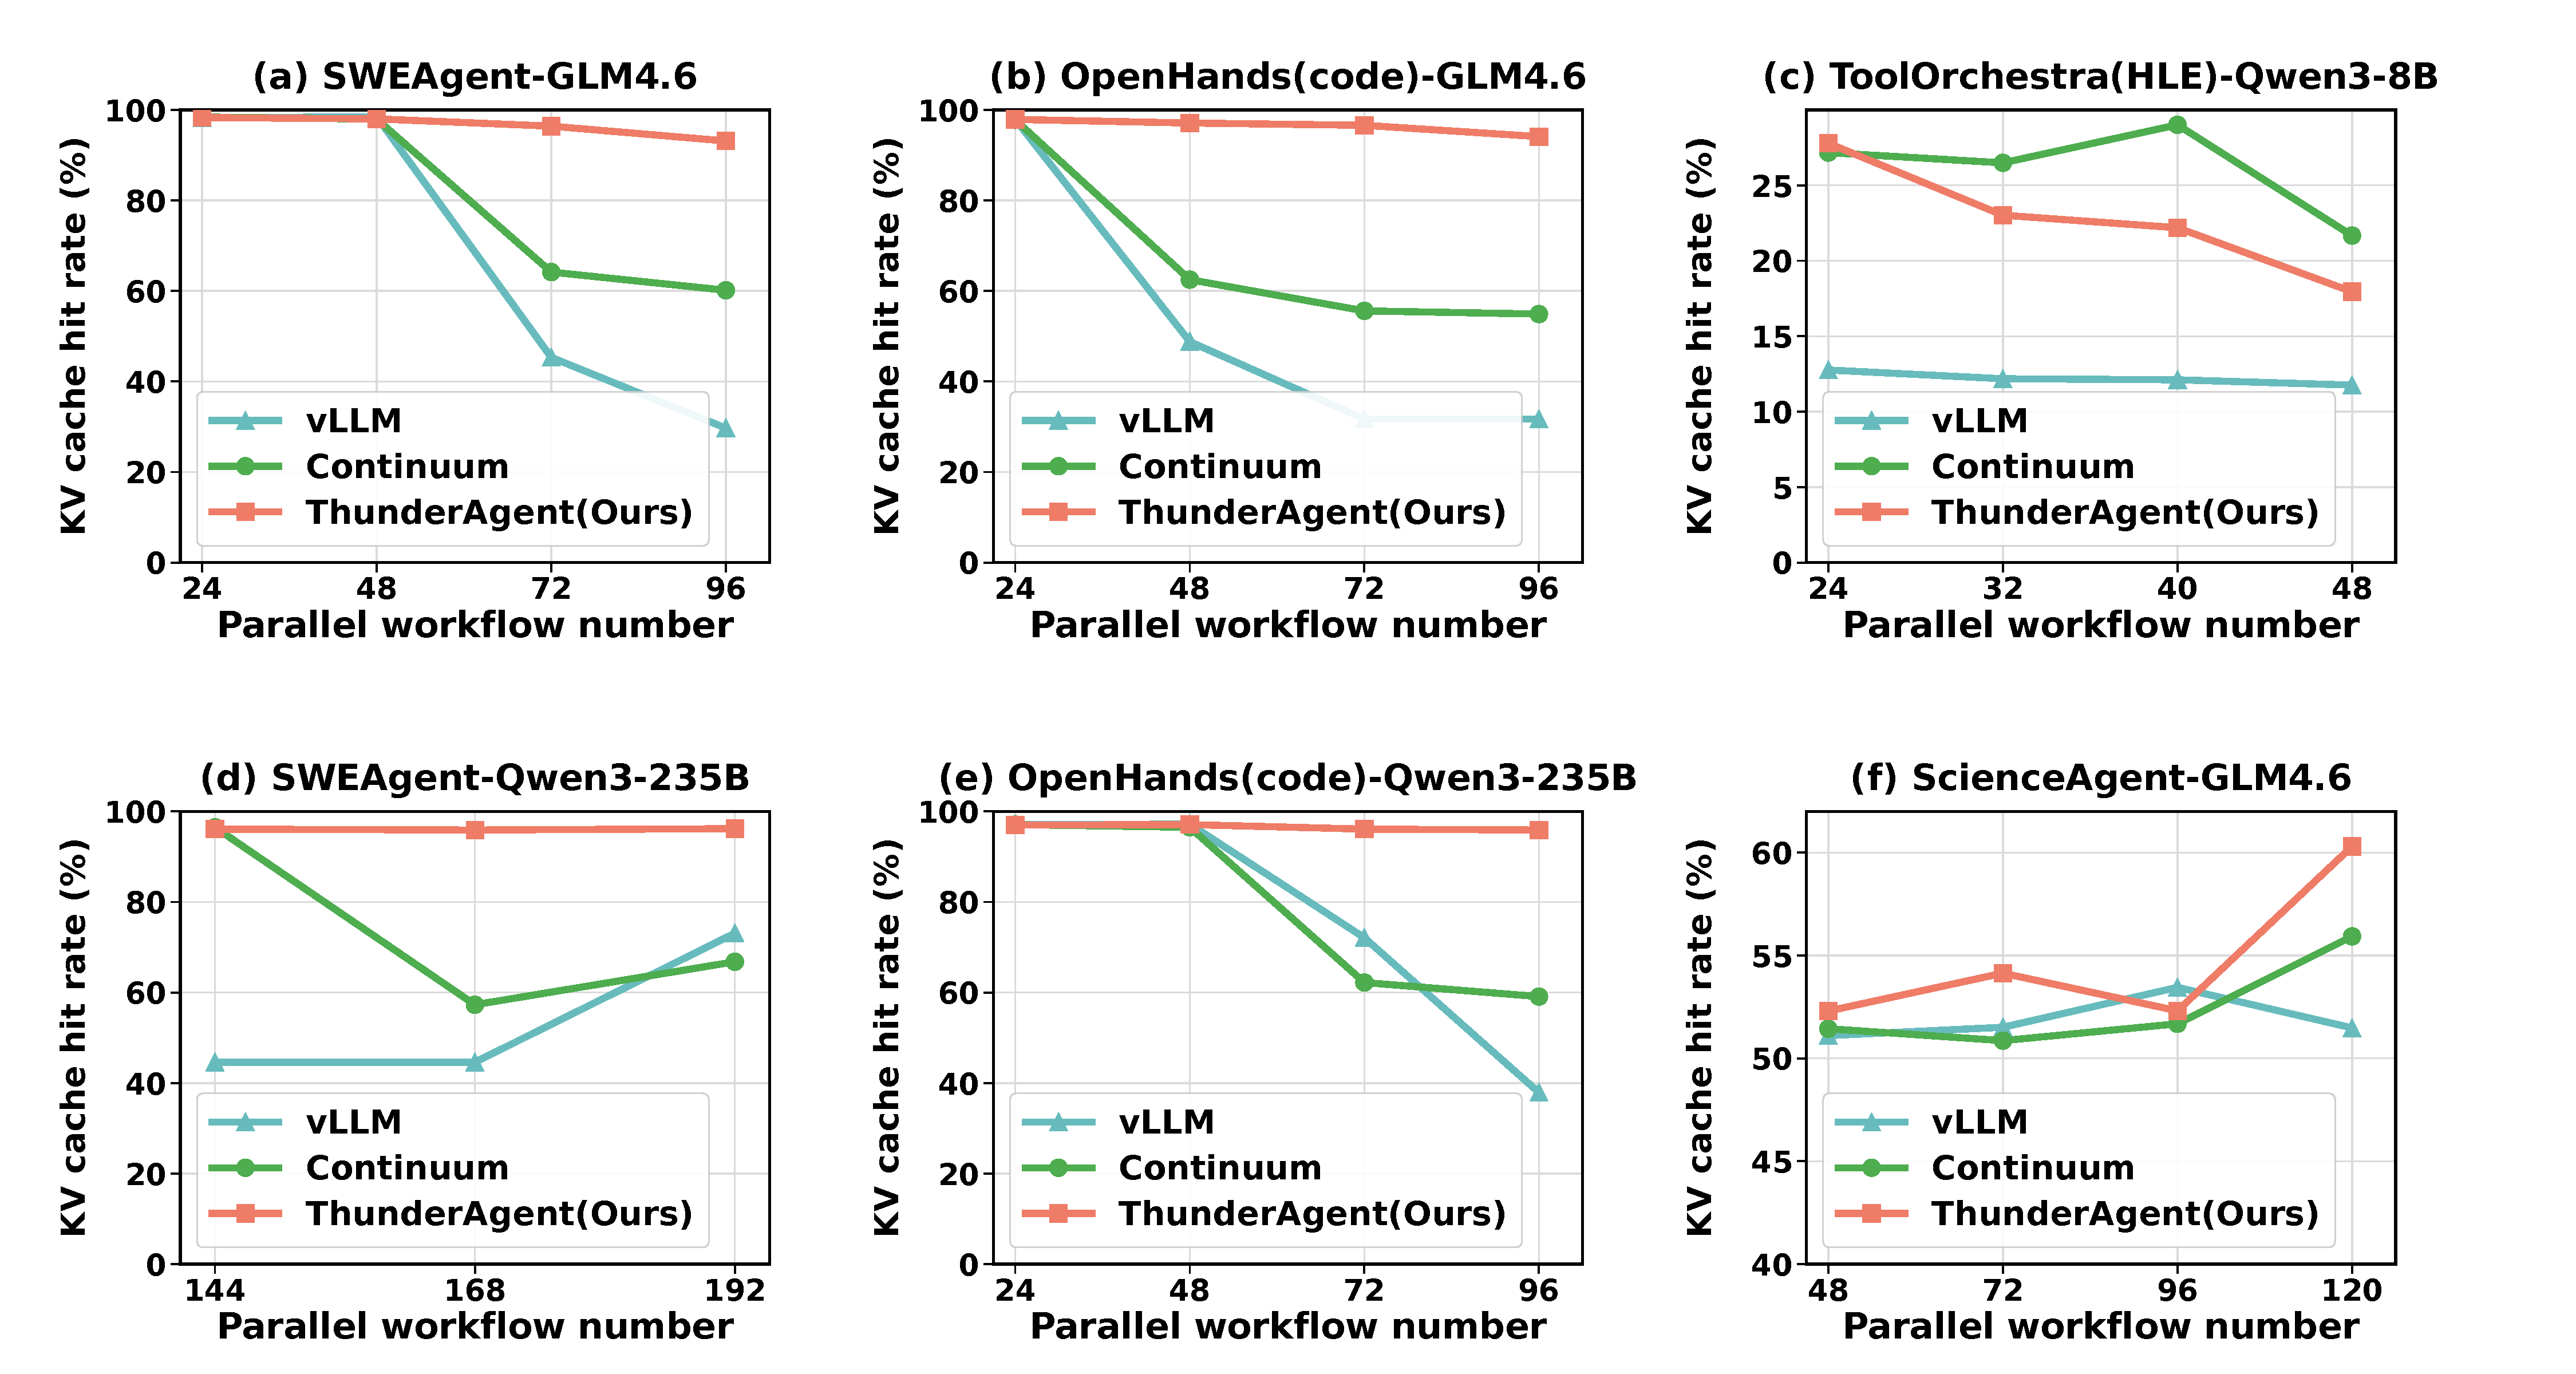
\includegraphics[width=\textwidth]{Figures/appendix_figs/kv_all.pdf}
  \caption{\textbf{KV 缓存命中率统计。} 对于工具调用时间可预测的工作流（a、b、d、e），\ouralg 达到接近最优（$\approx$100\%）的命中率；对于工具执行时间随机的工作流（c、f），\ouralg 会动态权衡命中率以减少空闲缓存。与 vLLM 和 Continuum 相比，它总体上实现了更高的 KV 缓存命中率。}
  \vspace{-1em}\label{fig:kv_hit_rate_data_statistics}
\end{figure*}
% We illustrate the throughput performance of~\ouralg compared to vLLM and Continuum in~\autoref{fig:eval_infer_result}, and \autoref{fig:kv_hit_rate_data_statistics} shows KV-cache hit rate among these settings. At high concurrency levels (e.g., 96 parallel programs), \ouralg demonstrates a substantial performance advantage. According to \autoref{fig:kv_hit_rate_data_statistics}, \ouralg reduces KV thrashing and maintains KV-cache hit rate by applying our scheduler discussed in \autoref{sec:scheduling_policy}. Even at lower concurrency (e.g., 24 parallel programs), \ouralg still achieves better throughput by reducing end-to-end latency and better tool resource management discussed in \autoref{sec:tool_resource}. Across different base models, agentic workflows, and datasets, \ouralg achieves a \textbf{1.48--3.58$\times$} speedup over vLLM and consistently outperforms Continuum by \textbf{1.17-3.31}$\times$.

\paragraph{高并发下的高吞吐量。}
\autoref{fig:eval_infer_result} 表明，\ouralg 在高并发级别（例如 96 个并行程序）下具有显著吞吐优势：在不同基础模型和数据集上，相比 vLLM 实现 \textbf{1.48--3.58$\times$} 加速，相比 Continuum 实现 \textbf{1.17--3.31$\times$} 加速。
这种收益来自我们的程序感知调度器，它能保持接近最优的 KV 缓存命中率（Mini-SWE-Bench 和 OpenHands 上约为 100\%，见 \autoref{fig:kv_hit_rate_data_statistics} a、b、d、e），并支持环境异步准备。相比之下，Continuum 在高并发下会出现性能下降。如 \autoref{fig:kv_hit_rate_data_statistics} 所示，它的 KV 缓存命中率从 $>$90\% 显著下降到 $\approx$60\%。这是因为当没有足够显存用于正在进行的请求解码时，Continuum 会在不同程序请求之间发生 KV 缓存驱逐，活动程序因争夺有限显存而引发系统抖动。

% \vspace{-1mm}
\paragraph{高并发的鲁棒性能。}
\ouralg 即使在并行工作流数量超出 GPU 显存限制时，也能保持最大可实现吞吐量。如 \autoref{fig:eval_infer_result} 所示，\ouralg 确保吞吐量随并行工作流数量增加仍保持稳定；而一旦工作负载超过显存限制，基线系统就会出现严重吞吐崩溃。在实际智能体服务中，由于智能体环境和工具执行持续时间具有随机性，通常无法静态确定最佳并行工作流数量，以在有限 KV 缓存抖动和缓存成本下最大化利用率。\ouralg 通过自动适应最大可用容量而无需手动调参来解决此问题，这是稳健实际部署的关键功能。

\paragraph{确定性和随机工具执行的鲁棒性。}
% \vspace{-1mm}
\ouralg 不仅在具有确定性工具模式的工作流中优于基线（\autoref{fig:eval_infer_result} a、b、d、e），而且也在高度随机的条件下（\autoref{fig:eval_infer_result} c、f）。
这来自我们的动态程序感知等待队列策略。vLLM 的请求感知调度器通常不会为处于执行阶段的程序保留显存，从而迫使系统频繁重新计算。相反，Continuum 会为所有暂停程序静态保留显存，并依赖工具执行时间预测；当工具调用很长且不可预测时，这会带来高昂的 $\text{Cost}_{\text{recompute}}$ 或 $\text{Cost}_{\text{caching}}$。
\ouralg 通过时间衰减函数平衡它们 $f(t)$，优先为工具调用时间短的程序保留 KV 缓存，同时抢先暂停工具执行时间长的程序，以防止内存浪费。
如图所示 \autoref{fig:kv_hit_rate_data_statistics} （右），虽然 \ouralg 在随机设置下，KV 缓存命中率低于 Continuum，它通过确保活动 GPU 利用率来实现更高的吞吐量。

% \ouralg not only outperforms vLLM and Continuum under agentic workflows that have deterministic and sufficient tool calls(a,b,d,e in \autoref{fig:eval_infer_result}), but also under conditions where tool calls are stochastic(c,f in \autoref{fig:eval_infer_result}). This is because vLLM applies a request-aware scheduler that has zero KV-cache space for acting programs. While Continuum does give every acting program enough space to place its KV-cache, this might cause great memory underutilization for GPU. \ouralg dynamically trade-off cost of caching and recompute by applying a time decay function $f(t)$ that erases caching places when GPUs are underutilized, but keeps the KV-cache programs that have short tool calls. Shown in(c,f in \autoref{fig:kv_hit_rate_data_statistics}), \ouralg has a lower KV cache hit rate than Continuum but maintains higher throughput.

% \vspace{-1mm}
% Beyond the performance gains,~\ouralg maintains maximum achievable throughput when the program number increases after maximize hardware utilization. In practical agentic serving and rollout, determining the optimal parallel program number that maximizes hardware utilization without triggering KV-cache thrashing, is often infeasible due to the stochastic nature of agent environments and tool execution durations. Unlike baseline systems where exceeding this unknown threshold leads to throughput collapse, \ouralg ensures that throughput remains approximately \textbf{non-decreasing} as the number of parallel programs increases. This capability allows the system to automatically utilize the maximum available hardware capacity without manual tuning, which is critical for real-world deployments handling dynamic agentic workloads.

% In the distributed setting, we evaluated GLM-4.6 rollout on a two-node H100 cluster over a three-hour duration, measuring throughput in reasoning steps per minute. \ouralg demonstrates effective scalability with the number of nodes, achieving a \textbf{1.79--3.92$\times$} throughput increase. This improvement is driven by the system's ability to balance memory utilization across backends and mitigate thrashing, validating the effectiveness of \ouralg for memory-intensive, distributed agentic RL workloads.
\begin{figure}[t!]  % 使用 figure* 让图片跨越两栏
    \centering
    \begin{subfigure}{0.40\textwidth}
        \centering
        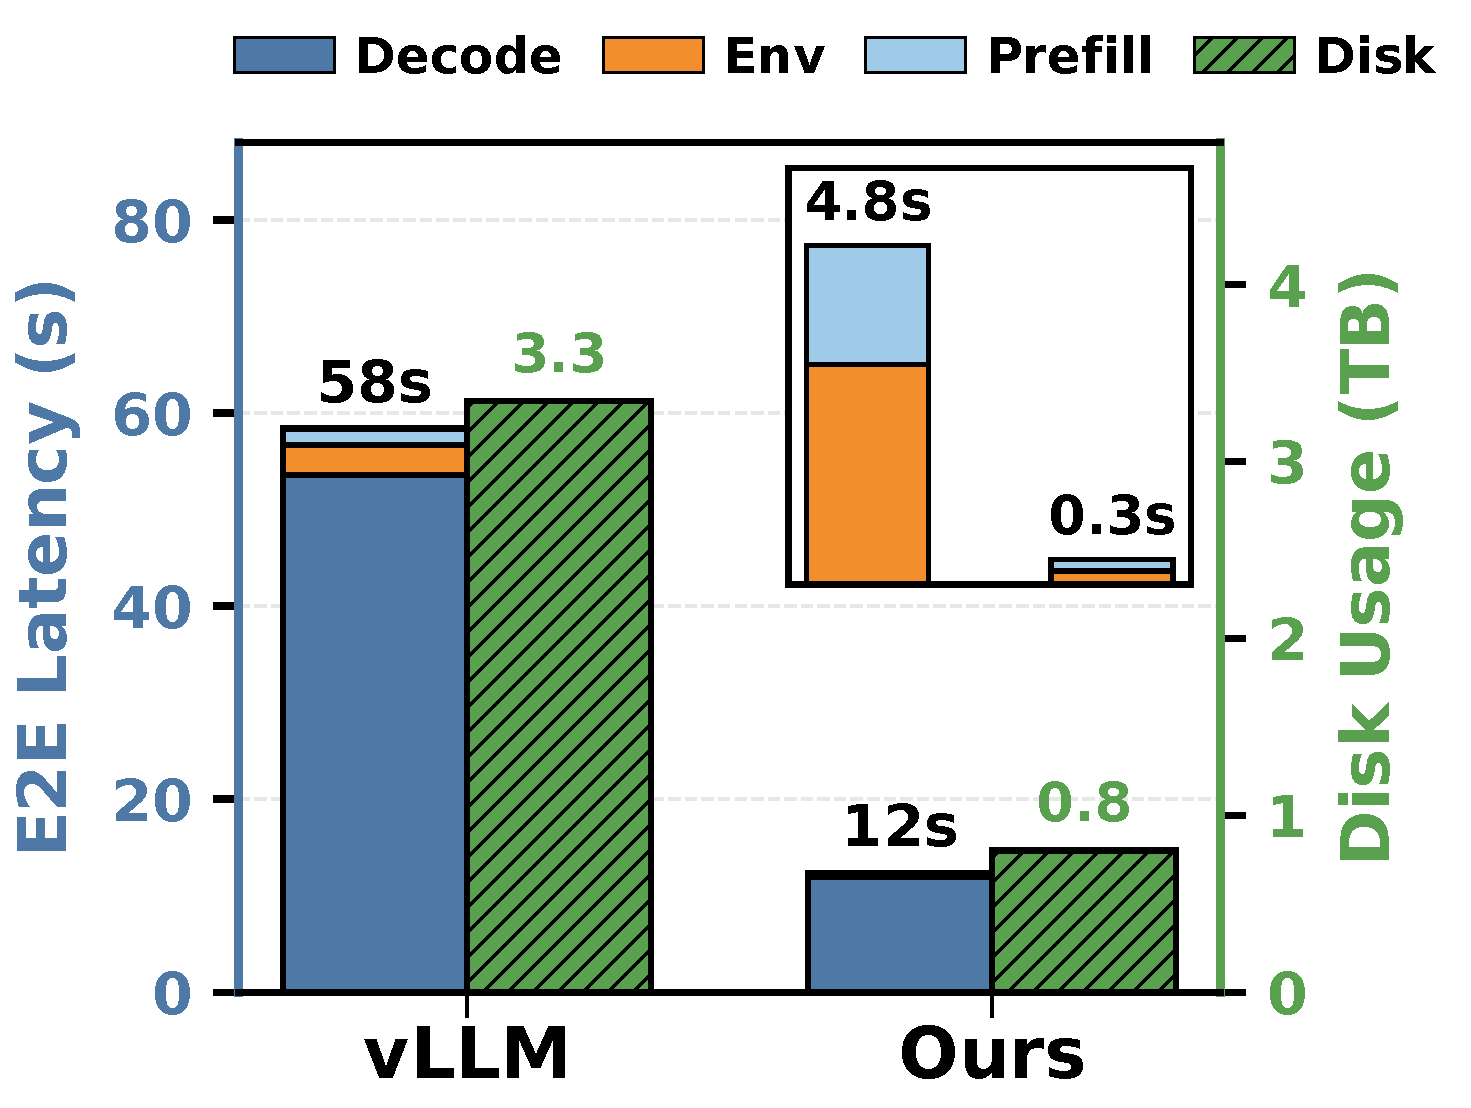
\includegraphics[width=0.99\textwidth]{Figures/e2e_breakdown.pdf}  % 替换为你的图片路径
        \caption{端到端延迟细分}
        \label{fig:breakdown}
    \end{subfigure}
    \begin{subfigure}{0.33\textwidth}
        \centering
        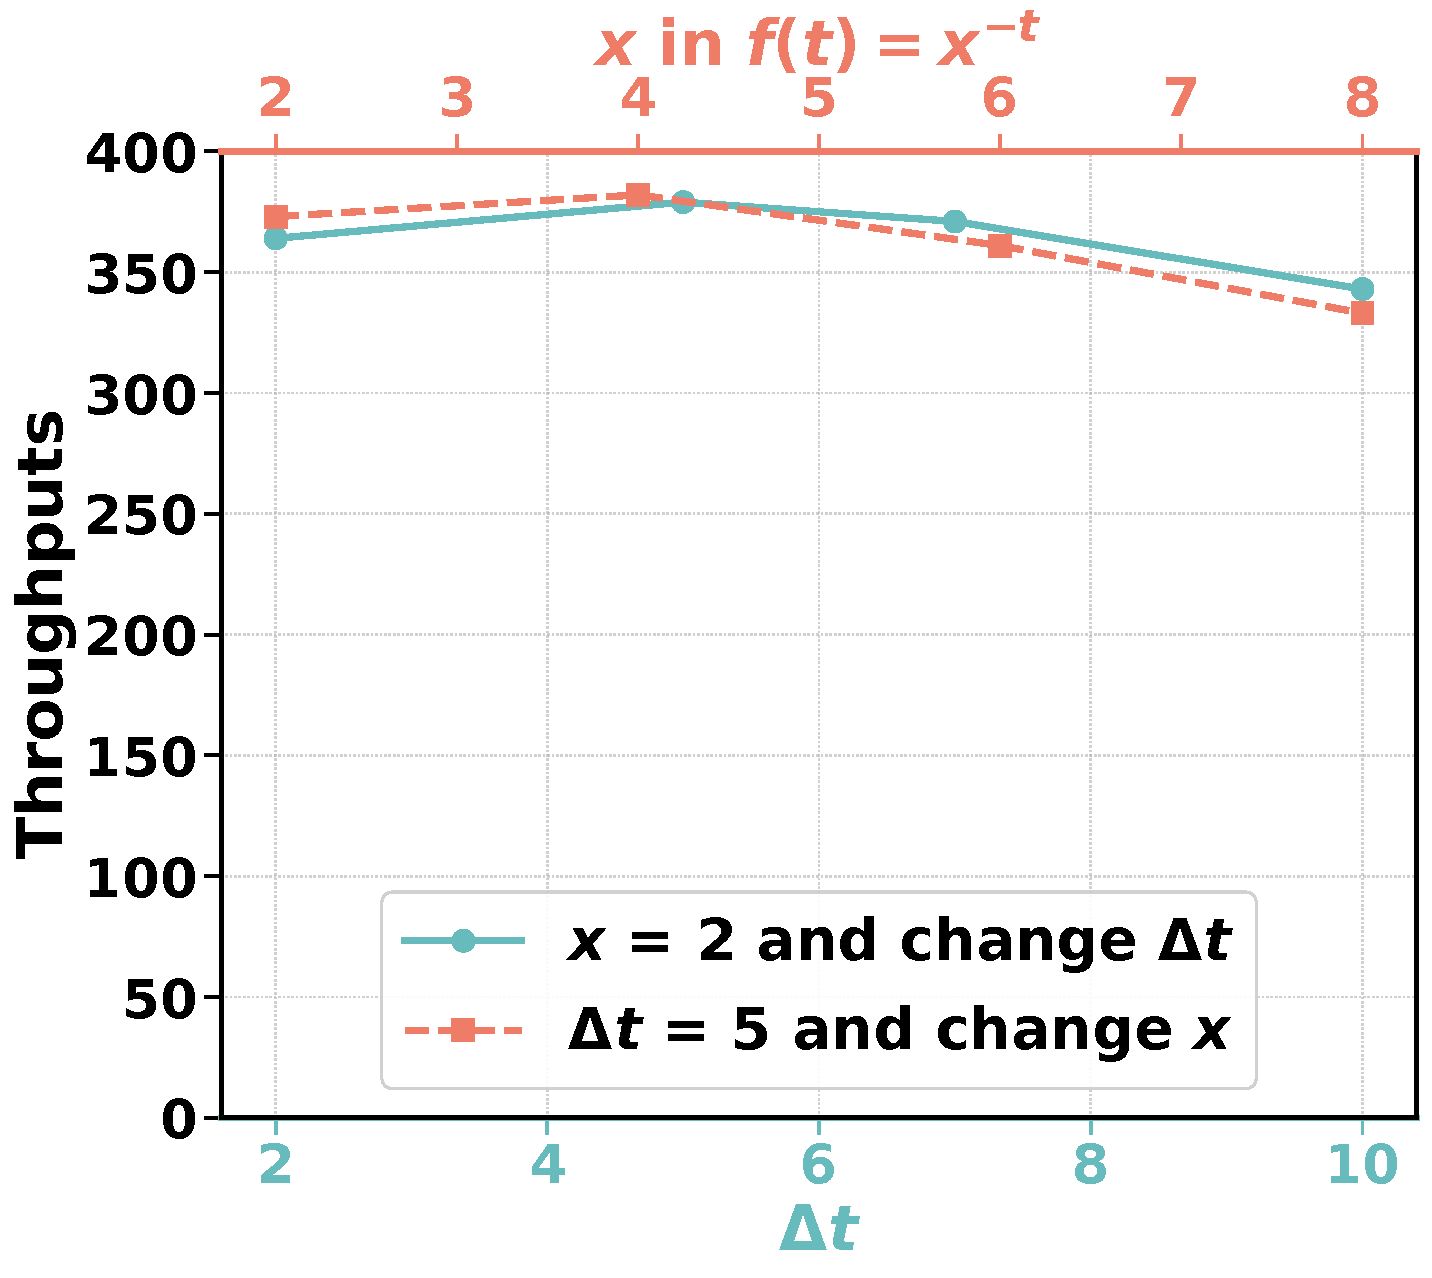
\includegraphics[width=0.99\textwidth]{Figures/parameter_ablation.pdf}  % 替换为你的图片路径
        \caption{消融 $\Delta t$ 和 f(t)}
        \label{fig:parameter_ablation}
    \end{subfigure}
    \caption{端到端延迟分解和参数敏感性的消融研究 \ouralg.}
    \label{fig:3}
    \vspace{-2mm}
\end{figure}


\vspace{-3mm}
\subsection{Rollout 评估结果}

% 紧凑版表格
\begin{wraptable}{r}{ 0.65\columnwidth}
\vspace{-1.1em}
\centering
\caption{\small 2$\times$H100 节点上的 \ouralg GLM-4.6 rollout（$N=144$）。}
\vspace{-0.3em}
\label{tab:blocksize_ablation}
\resizebox{\linewidth}{!}{\setlength{\tabcolsep}{3mm}{
\begin{tabular}{llr}
\toprule
Workflow & Serving System & Throughput \\
\midrule
mini-SWEAgent & vLLM + Gateway & 375.4 \\
mini-SWEAgent & \ouralg & 671.8 (\textbf{1.79$\times$}) \\
OpenHands & vLLM + Gateway & 69.1 \\
OpenHands & \ouralg & 270.8 (\textbf{3.92$\times$}) \\
\bottomrule
\end{tabular}}}
\end{wraptable}

我们在两节点 H100 集群上使用 GLM-4.6 评估 RL rollout（持续时间 3 小时）。\autoref{tab:blocksize_ablation} 表明，\ouralg 保持了有效可扩展性，相比 vLLM + Gateway 基线实现 \textbf{1.79--3.92$\times$} 吞吐提升，说明它非常适合显存密集型分布式强化学习工作负载。
% 删掉了 "This improvement is driven by..." 整句

\vspace{-2mm}
\subsection{消融研究}\label{app:ablation_study}
\paragraph{端到端延迟细分。}
\autoref{fig:breakdown} 分解了 OpenHands rollout 的平均端到端延迟。吞吐量提升主要来自 \textbf{预填充和解码延迟} 的降低。此外，工具资源管理策略（\autoref{sec:tool_resource}) 贡献了约 \textbf{10\%} 的延迟改善，并带来 \textbf{4.2$\times$} 的磁盘空间节省。每步端到端延迟见 \autoref{app:e2e}.
% 删掉了 "by reducing KV-cache thrashing..." 重复解释
% \begin{figure}[t!]  % 使用 figure* 让图片跨越两栏
%     \centering
%     \begin{subfigure}{0.40\textwidth}
%         \centering
%         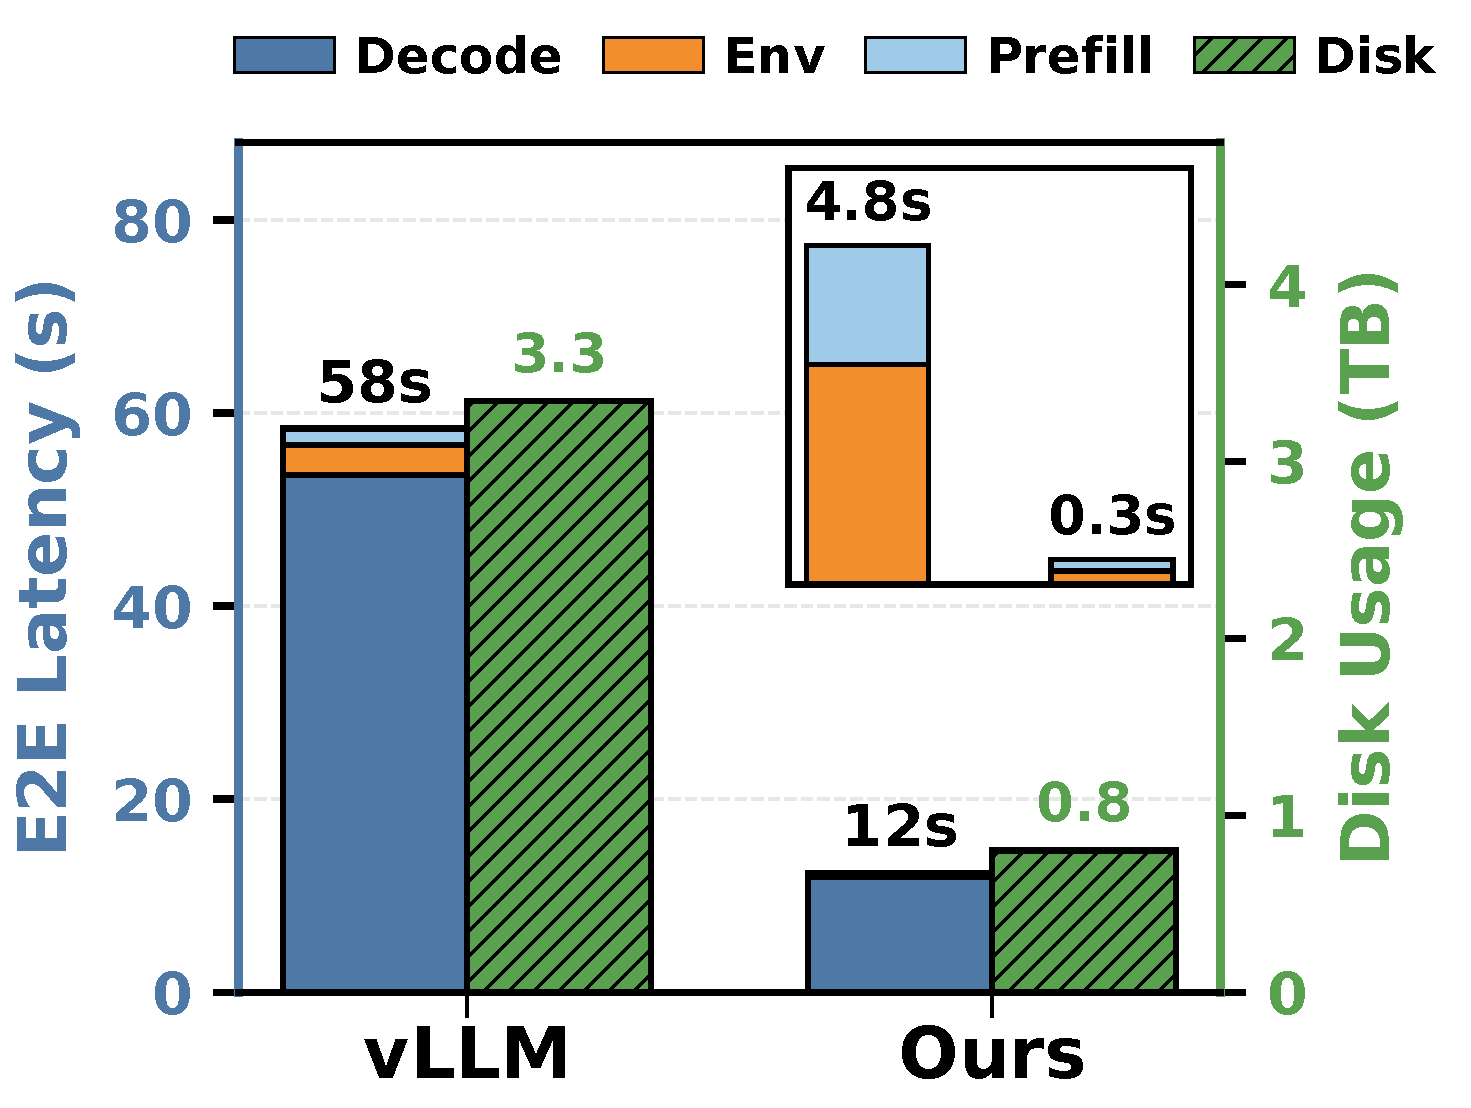
\includegraphics[width=0.99\textwidth]{Figures/e2e_breakdown.pdf}  % 替换为你的图片路径
%         \caption{End-to-end Latency}
%         \label{fig:breakdown}
%     \end{subfigure}
%     \begin{subfigure}{0.33\textwidth}
%         \centering
%         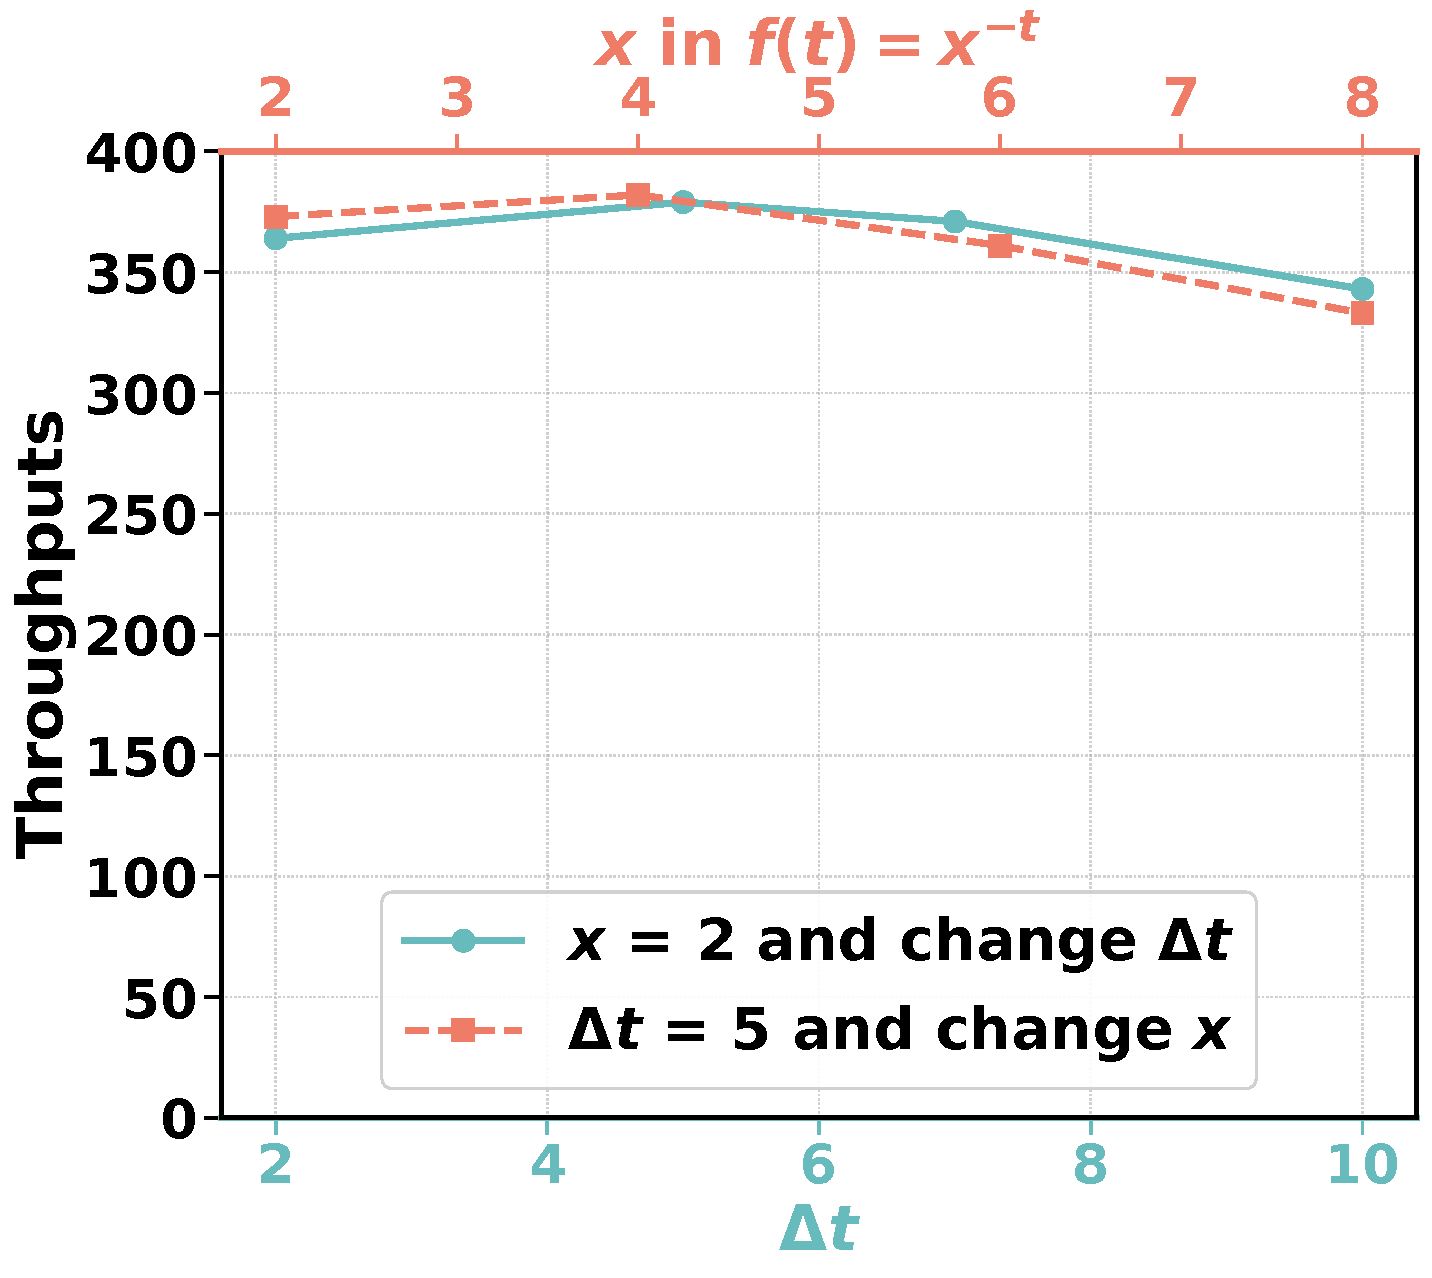
\includegraphics[width=0.99\textwidth]{Figures/parameter_ablation.pdf}  % 替换为你的图片路径
%         \caption{Ablation of $\Delta t$ and f(t)}
%         \label{fig:parameter_ablation}
%     \end{subfigure}
%     \caption{Ablation study of agentic RL rollout and parameter sensitivity of \ouralg.}
%     \label{fig:3}
% \end{figure}

\paragraph{消融开启 $\Delta t$ 和 f(t)。} 我们研究检测周期的灵敏度 $\Delta t$ 和衰减功能 $f(t) = x^{-t}$. \autoref{fig:parameter_ablation}
 节目 \ouralg 在单个 H100 节点上以 GLM-4.6 作为基本模型离线服务mini-SWEAgent。我们观察到 \ouralg 在不同参数设置下保持高吞吐量，证明了我们方法的稳健性。进一步增加 $\Delta t$ 可能会降低 KV 缓存命中率，从而降低吞吐量，因为检测过程中可能会发生抖动。另外，增加 $x$ 在 $f(t)$ 允许更积极地驱逐执行程序，这些程序通过重新计算成本来降低缓存成本。这会降低智能体程序的吞吐量
工具执行时间短会被过早驱逐。% \textbf{Ablation study on KV cache offloading.}
% We investigated KV cache offloading via LMCache as a potential remedy for capacity constraints. While offloading theoretically extends effective memory space by utilizing CPU or disk storage, our implementation with vLLM+LMCache reveals a critical bottleneck: the PCIe bandwidth is insufficient to sustain the high-frequency context switching and large-volume data transfers inherent to agentic workloads. As shown in \autoref{fig:kv_offload}, when serving GLM-4.6 with mini-SWEAgent, the latency penalty from frequent swap-in/swap-out operations negates the capacity benefits, resulting in severe throughput degradation under heavy loads.

% \textbf{Ablation study on Prefill-Decode (PD) disaggregation.}
% We also explored PD disaggregation, a standard optimization for chatbot serving designed to isolate the decoding phase from prefill interference. However, for agentic workloads which are characterized by continuous context growth, we observe that PD disaggregation \textbf{\textit{exacerbates}} thrashing. By physically partitioning the cluster into prefill-only and decode-only nodes, the effective HBM pool available for handling prefill is significantly smaller than in a unified architecture. This memory fragmentation causes the system to hit capacity limits and trigger thrashing at much lower concurrency levels, as shown in \autoref{fig:pd disaggregation}. \textbf{These results demonstrate that generic architectural optimizations cannot substitute for a program-centric scheduler that actively manages the working set.}
